\documentclass{article}
\usepackage[utf8]{inputenc}
\usepackage{listings}
\usepackage{graphicx}
\usepackage{caption}
\usepackage{subfig}
\begin{document}

\section{Giving the Greenhouse a realistic view}
\subsection{The camera view}
The Camera view shows the current scene as seen from the active camera’s viewpoint. It can also be used to show how the scene will look like when it is rendered. Once activated and locked to the view, the camera can be moved around the scene to capture shots of the objects from different views and perspectives.
\newline

\begin{figure}[htp]
    \centering
    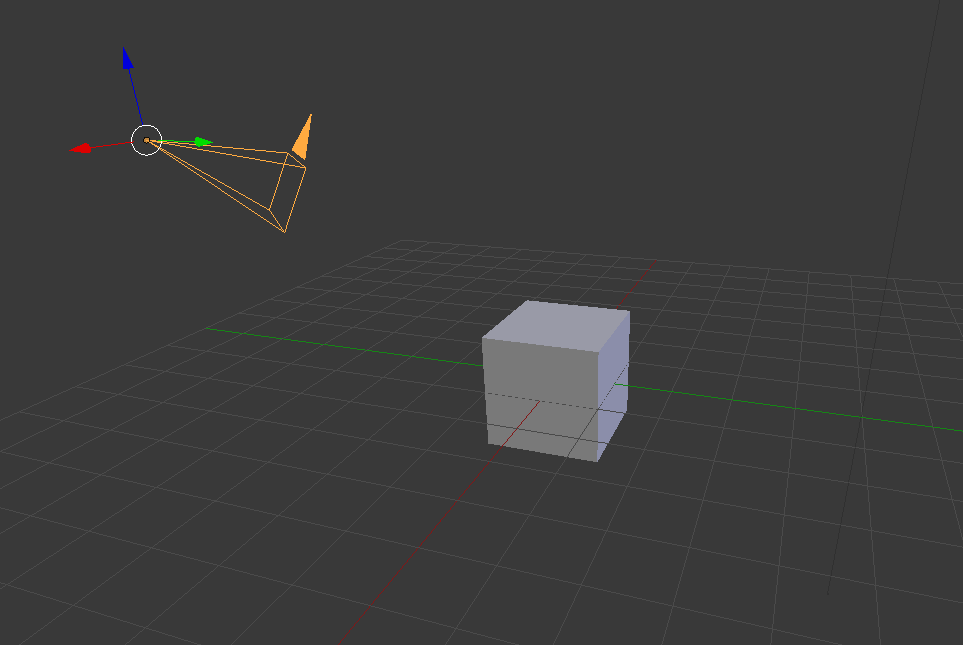
\includegraphics[width=6cm]{Camera.PNG}
    \caption{Camera Position}
\end{figure}

\subsection{The rendering engines}
Rendering is the process of turning a 3D scene into a 2D image.There are three rendering engines in Blender:
\begin{itemize}
\item Cycles
\item Eevee
\item Workbench
\end{itemize}
The result of each rendering engine depends on various features such as  cameras, lights and materials. These features are supported by both \textbf{Eevee} and \textbf{Cycles}. However there are some features which are only supported in one or another.
\newline
\par\textbf{Cycles} is Blender’s physically-based path ray tracer for production rendering. It is designed to provide physically based results out-of-the-box, with artistic control and flexible shading nodes for production needs.
There are four different light ray types supported by \textbf{Cycles}:
\begin{itemize}
\item From Camera
\item Generated by a reflection off a surface
\item Generated by a transmission through a surface
\item The ray is used for shadows
\end{itemize} \par
  
\textbf{Eevee} is Blender’s real-time render engine. Unlike Cycles, it is not a ray tracing render engine, and uses a process called \textbf{Rasterization}. This process estimates the way light interacts with objects and materials using numerous algorithms.
\newline
\begin{figure}[htp]
    \centering
    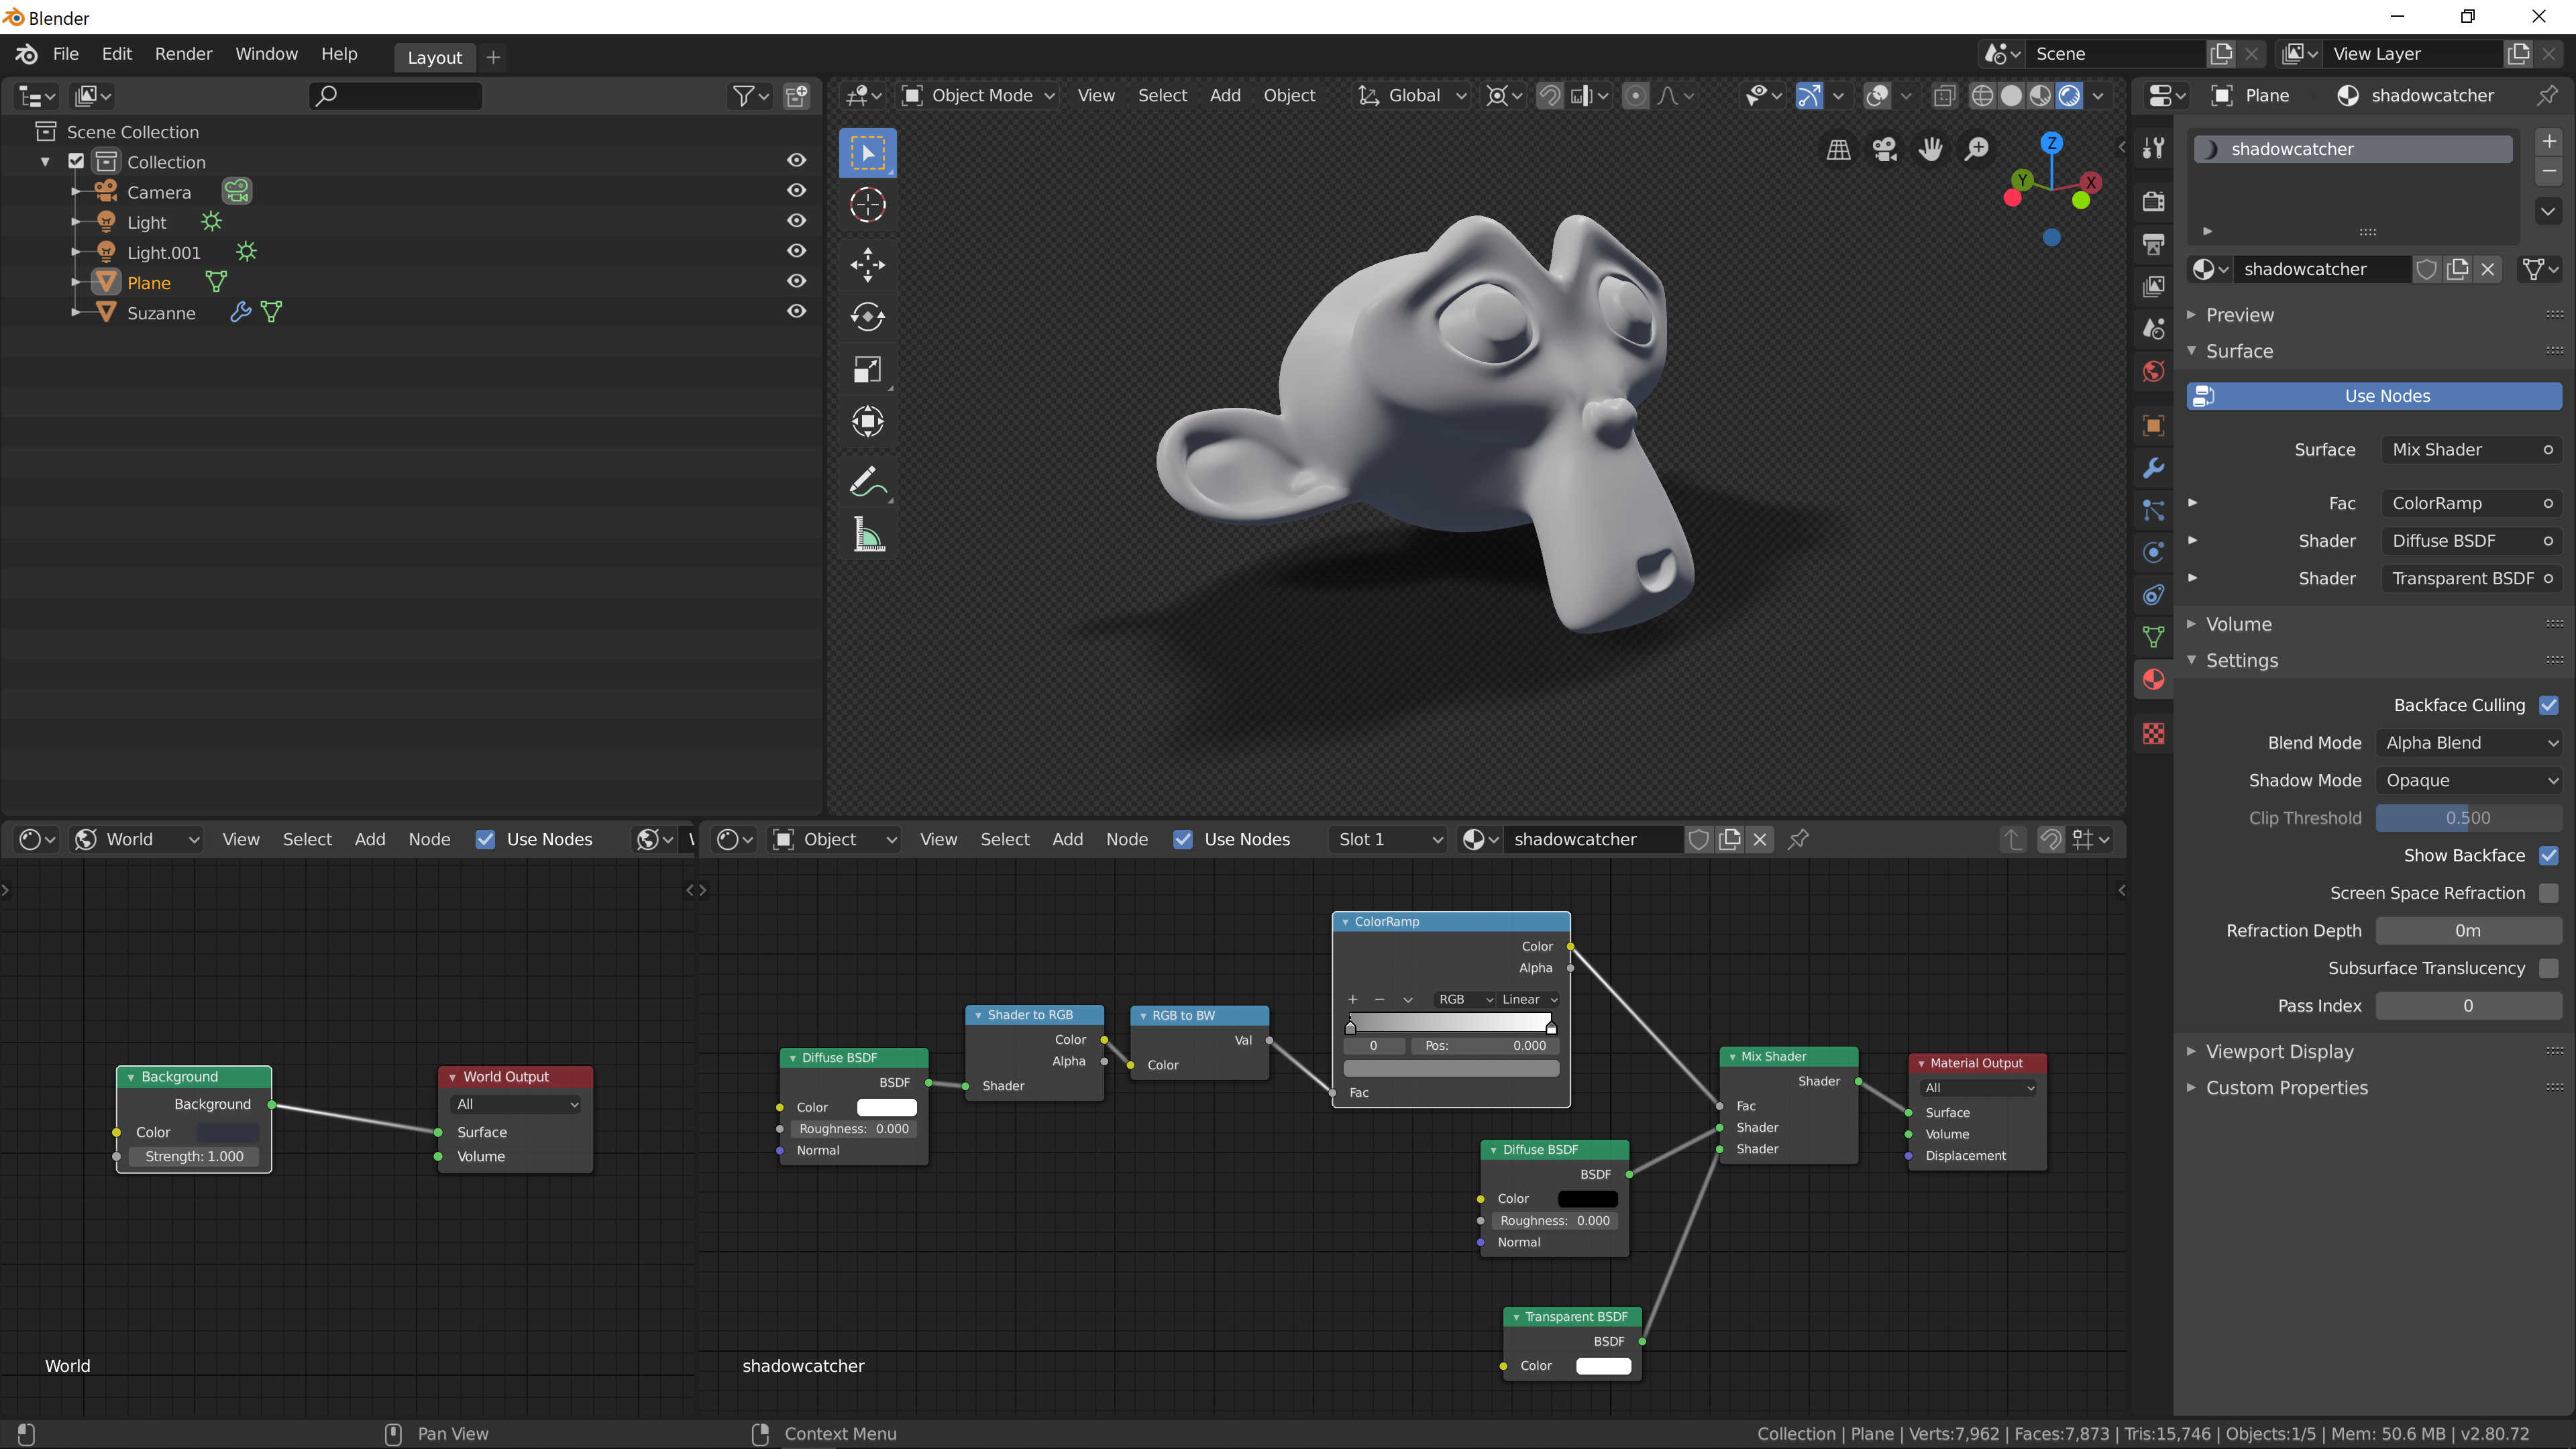
\includegraphics[width=6cm]{EEVEE.jpg}
    \caption{eevee rendering Engine}
\end{figure}
\par
For fast rendering during modeling and animation preview, \textbf{Workbench} can be used. \textbf{Workbench} supports assigning random colors to objects to make each of them visually distinct. Other coloring mechanisms also exist, including; materials, vertex colors, and textures. Its primary task is to display a scene in the 3D Viewport when it is being worked on, and not rendering the final image for a project.
\newline
\par
\subsection{Texturing}
Texturing is one of the most important stages in rendering. Textures are applied to the object, or to be more precise, object's mesh to create the appearance of the object and give a the materialistic view to it. A mesh is a collection of vertices, edges, and faces that describe the shape of a 3D object. The advantage of using texture vs. image is that it is not necessary to place the image on each coordination to make it look 3D. Scripting is used to automate the process of creating and placing nets under each plant.
\newline
\par
\subsection{How it is done}
A texture is downloaded from an open-source online website such as \textit{texture.com}. A plane mesh is created under each Plant. Since the mesh has a primitive shape (e.g. circle, cube, cylinder…), it can be edited to create a larger, more complex shape. In shading mode the texture is added as a node, and then is connected to the mapping of \textbf{textureCoordinate} and \textbf{principledBSDF}.
\newline
\par
Features such as saturation, color or others are added as a node, and connected to the texture node. Changing the values of these nodes can change the properties such as light, color, ... of the texture. The following python code applies the texture to each plane:

\begin{lstlisting}
    plane = bpy.context.selected_objects[0]
    print('\nPlane coordinates: X: ' + 
           str(plane.location.x) + 
           ' Y:' + 
           str(plane.location.y) + '\n')
    mat = bpy.data.materials.new('materialA')
    bpy.context.object.data.materials.append(mat)
    mat.use_nodes = True
\end{lstlisting}

Linked nodes using BSDF principal are defined, which is used for shading textures:
\newline
\begin{lstlisting}
    bsdf = mat.node_tree.nodes["Principled BSDF"]
\end{lstlisting}
\begin{figure}[htp]
\centering
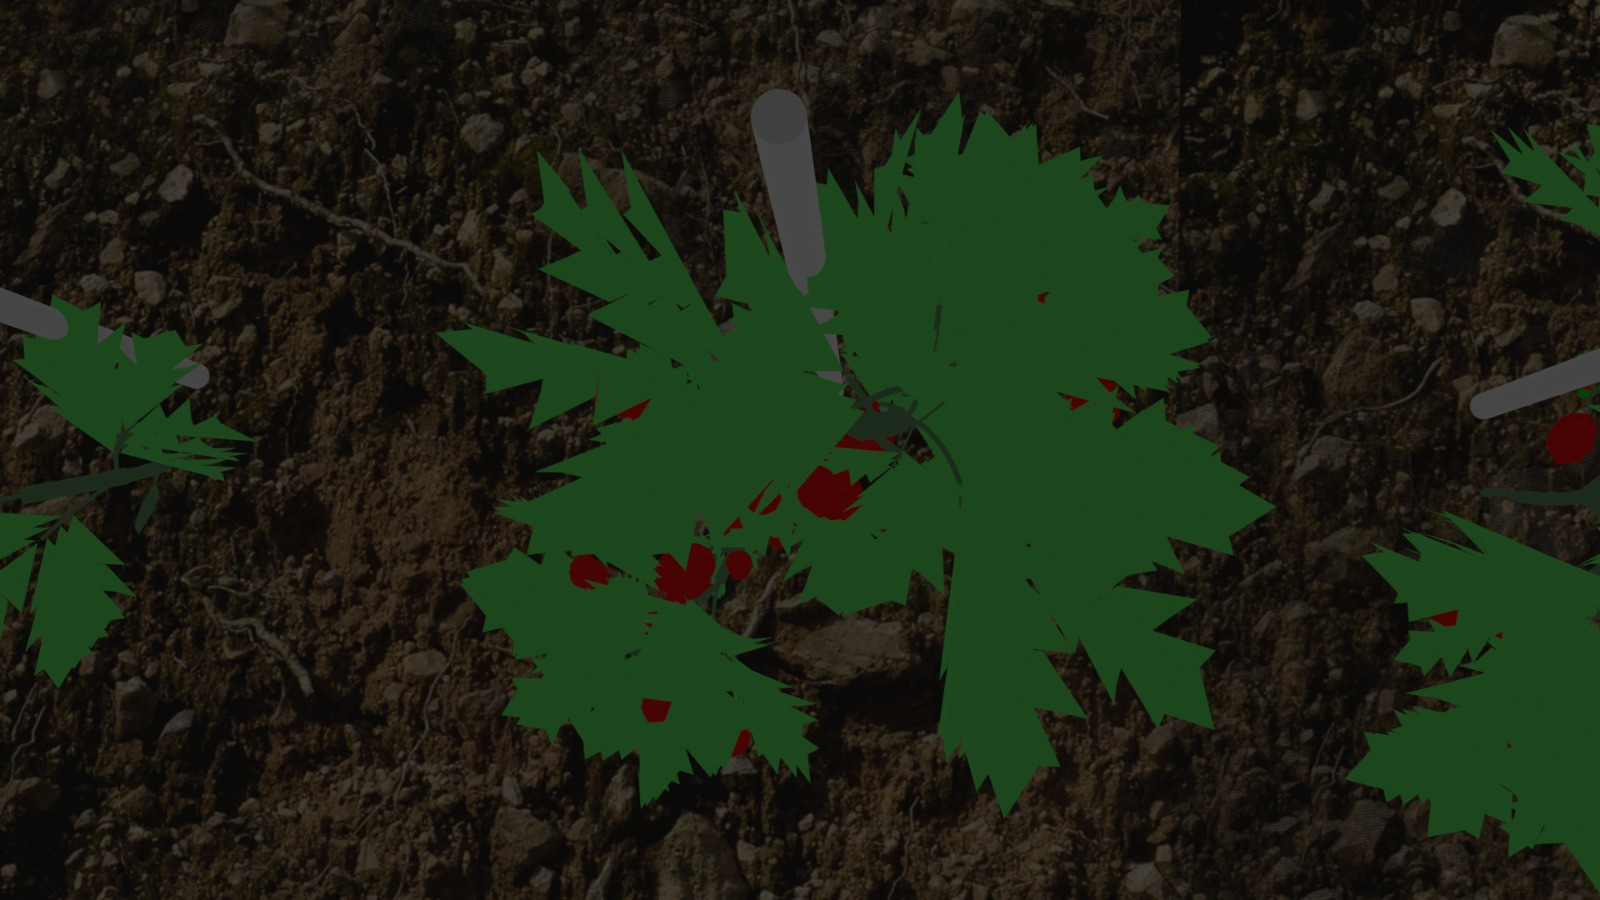
\includegraphics[width=6cm]{Texture.jpeg}
\caption{Imported Texture under the plant}
\end{figure}

\subsubsection{The lighting}
\par
The name of the light in Blender 2.8 is changed from ``lamp'' to ``light''. There are 4 types of light :
  \begin{itemize}

  \item\textbf{Point light} is a directional point of light. The light power and size can be easily changed. The power is in Watt and the point light with a larger size has softer shadows and specular highlights. \newline
 \begin{figure}[htp]
            \centering
            \includegraphics[width=5cm]{point.png}
            \captionof{figure}{Point light}
        \end{figure}

  \item\textbf{Sun light} provides light of constant intensity emitted in a single direction from infinity far away. It is represented by a encircled black dot with dots emitting from it. \par
 \begin{figure}[htp]
           \centering
            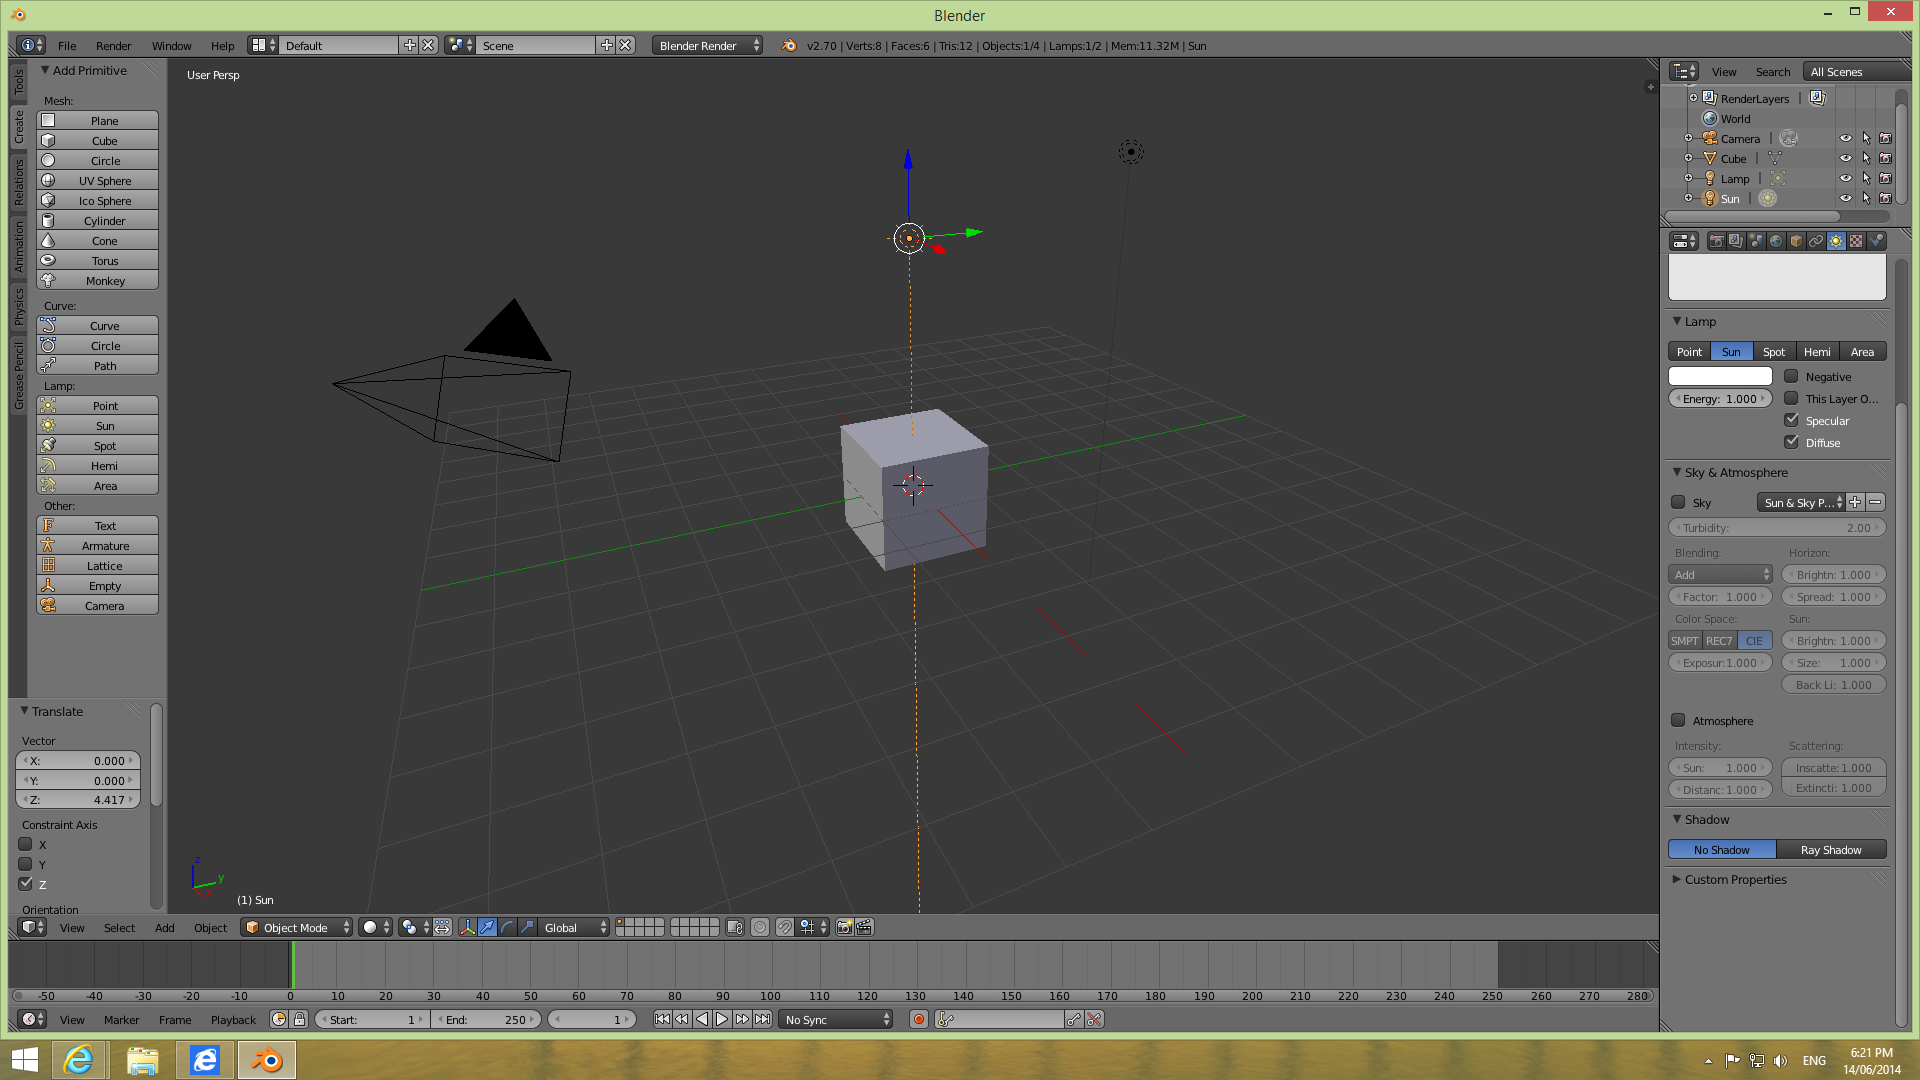
\includegraphics[width=6cm]{Sun.png}
            \captionof{figure}{Sun light}
           \end{figure}

  \item\textbf{Area light} simulates light originating from a surface emitter. For example, a TV screen or office neon lights. \newline
 \begin{figure}[htp]
           \centering
            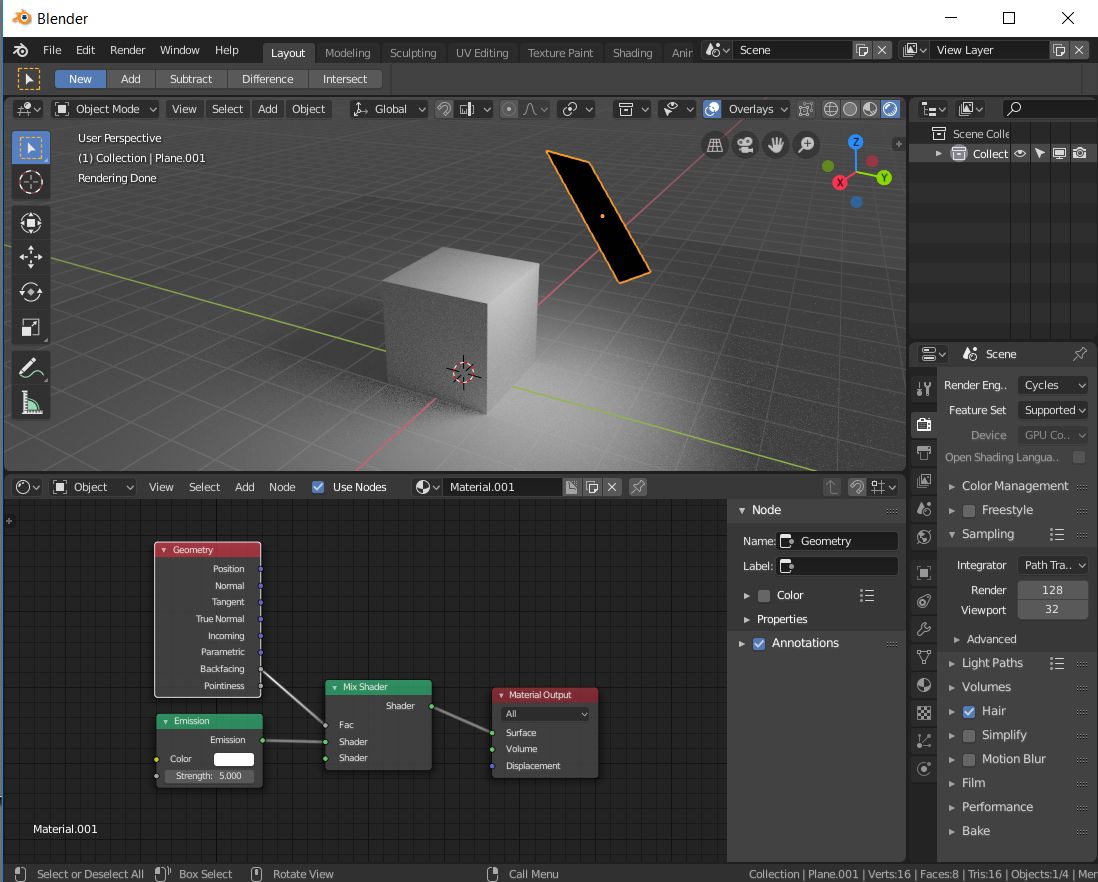
\includegraphics[width=6cm]{Area.png}
            \captionof{figure}{Area light}
            
            \end{figure}
\item\textbf{Spot light} is a cone shape beam of light. Just like point light the power of the light is in Watt and the larger size has softer shadows and specular highlights. This light is used in the project, because it is the only light type with a shadow, which eliminates the need to define shadows as texture separately.
 \end{itemize}
 
 \begin{figure}[htp]
          \centering
            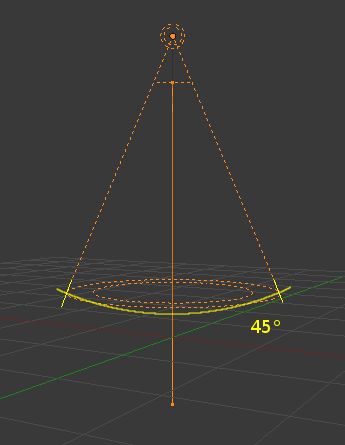
\includegraphics[width=6cm]{spot.png}
            \captionof{figure}{Spot light}
\end{figure}

 
\par
\newline
\subsection{The shadow}
A shadow map is a texture which stores the nearest occluder from the light position. The properties for shadows are :
  \begin{itemize}
  \item Cube size, used in Point, Area and Spot light. Higher shadow map size gives sharper shadows.
  \item Cascade size will only used in Sun light.
  \item High Bitdepth reduces some artifacts due to float imprecision inside the shadow maps.
  \item Soft shadows randomizes shadow maps origin to create soft shadows.
  \item Light Threshold. Setup time will saved due to computing the distance automatically based on a light threshold. 
 \end{itemize}
 
The following python code applies the light above each plane:

\begin{lstlisting}
    texImage = mat.node_tree.nodes.new('ShaderNodeTexImage')
    texImage.image = bpy.data.images.
                     load("C:/My Documents/Blender/Textur.jpg")
    mat.node_tree.links.new(bsdf.inputs['Base Color'],
                            texImage.outputs['Color'])
    \end{lstlisting}
     \newpage  \begin{figure}[htp]%
    \centering
     \subfloat[Plant after applying light- side]{{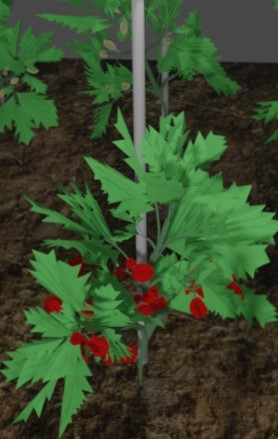
\includegraphics[width=5cm]{Side.jpeg} }}%
    \qquad
    \subfloat[Plant after applying light- up]{{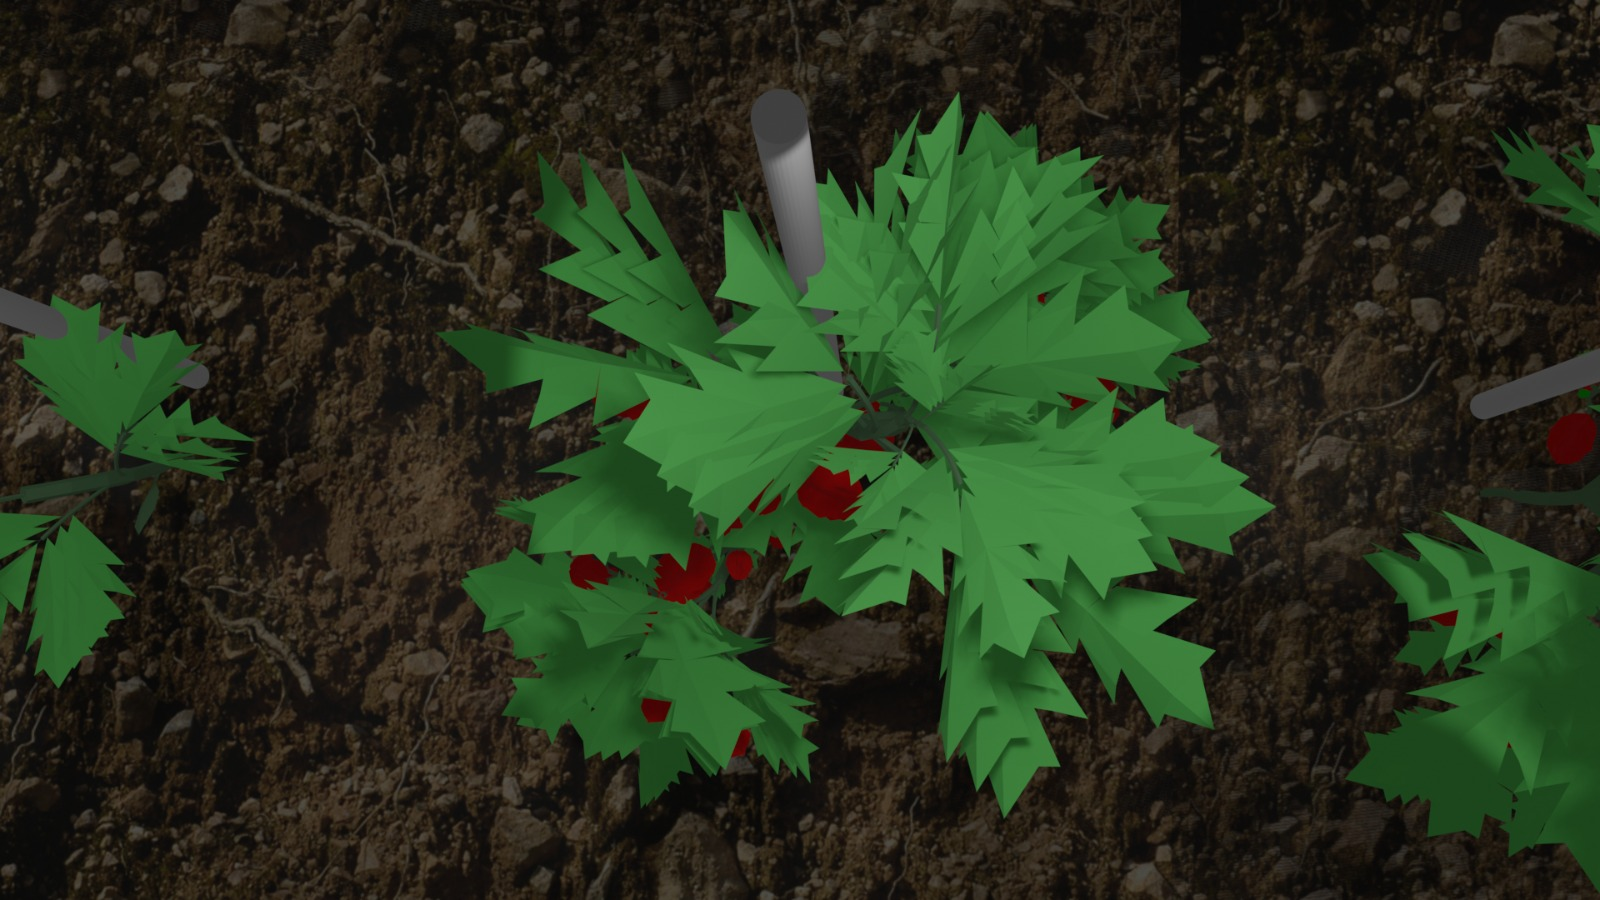
\includegraphics[width=5cm]{up.jpeg} }}%
\end{figure}

\end{document}
